\documentclass[12pt]{article}

\usepackage[utf8]{inputenc}
\usepackage[T1]{fontenc}
\usepackage[spanish]{babel}
\addto\captionsspanish{\renewcommand{\tablename}{Tabla}}

\usepackage[margin=2.5cm]{geometry}
\usepackage{graphicx}
\graphicspath{{imgs/}}

\usepackage[colorlinks=true, urlcolor=blue]{hyperref}

\title{Actividad 2: Laboratorio\\[1ex] \large Visualización Interactiva de la Información}
\author{David Vicente Moya}
\date{\today}

\begin{document}
\maketitle

\section{Causas de muerte más comunes}

\begin{figure}[ht]
    \centering
    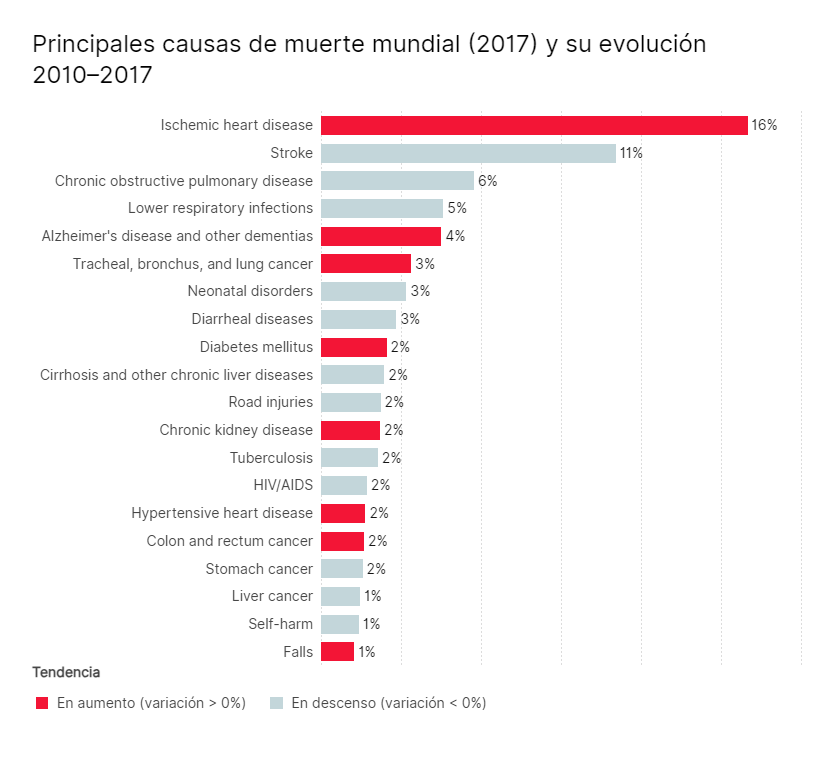
\includegraphics[width=0.8\textwidth]{parte1.png}
    \caption{Gráfico generado para identificar cuáles son las causas de fallecimiento 
    más importantes y si se trata de causas en aumento o en descenso.}
    \label{fig:parte1}
\end{figure}

\subsection{Descripción del dataset}

En la primera parte de la actividad se haabían marcado los obtjetivos de estructurar 
y preparar los datos provistos~\cite{causeofdeath} para, posteriormente, generar un 
gráfico que permita identificar cuáles son las causas de muerte más comunes y si 
se trata de causas en aumento o en descenso.

\subsection{Procesado de datos}

Los datos contenidos en el dataset~\cite{causeofdeath} se han procesado utilizando 
Excel. Se han eliminado las columnas que contenían un único valor (\texttt{Location}, 
\texttt{Age} y \texttt{Sex}), ya que no aportaban nada a la visualización. Además, se 
han pivotado los datos para separar en dos columnas el porcentaje total de muertes en 
2017 y el porcentaje anual de cambio 2010-2017. Los datos se han representado en una gráfica de barras, done se ha coloreado las barras 
de rojo para las causas de muerte que han visto un aumento en su porcentaje anual de 
cambio.

\subsection{Interpretación de resultados}

En la Figura~\ref{fig:parte1} destacan la \textbf{cardiopatía isquémica} y el 
\textbf{ataque isquémico} como las causas principales de muerte en 2017, juntas suponen 
más de un quinta parte del total de causas de muerte. Junto con la enfermedad cardíaca 
hipertensiva conforman el 29\% de las causas de muerte 
en 2017, estando las tres estrechamente relacionadas con enfermedades cardiovasculares y
problemas del corazón en general. Otro aspecto destacable de los resultados es la presencia, en forma de diferentes tipos, 
de cáncer entre las causas de muerte más comunes.

\section{Destinos turísticos más populares}

\begin{figure}[ht]
    \centering
    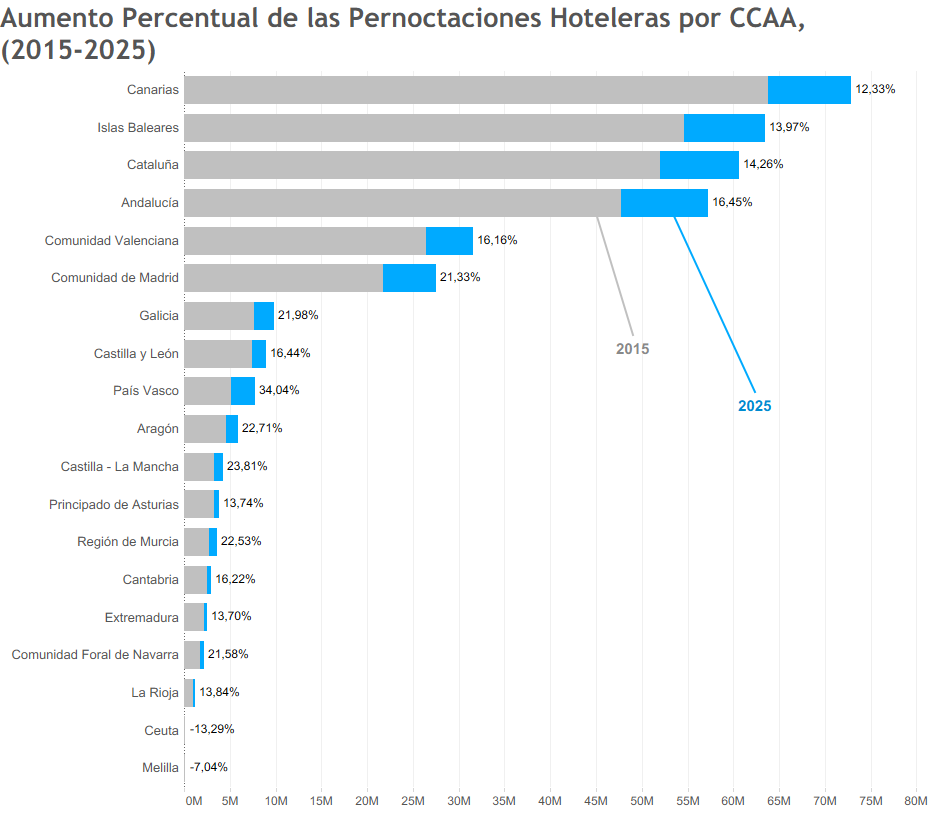
\includegraphics[width=0.8\textwidth]{parte2.png}
    \caption{Gráfico generado para identificar cuáles son los destinos turísticos más 
    populares y si la popularidad de estos destinos está en aumento o en descenso.}
    \label{fig:parte2}
\end{figure}

\begin{figure}[ht]
    \centering
    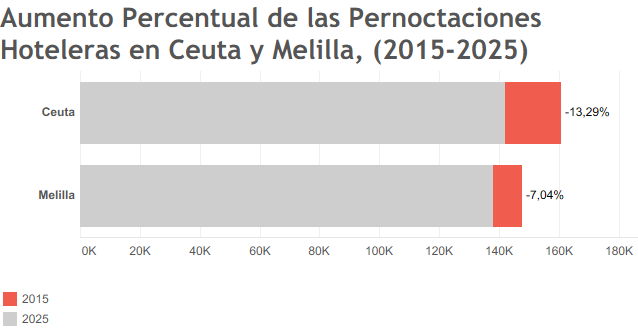
\includegraphics[width=0.6\textwidth]{parte2b.png}
    \caption{Detalle la evolución de la 
    popularidad de Ceuta y Melilla como destinos turísticos.}
    \label{fig:parte2b}
\end{figure}

\subsection{Descripción del dataset}

Para la segunda parte de la actividad tenía como objetivo buscar, estructurar y 
preparar un dataset que permita representar gráficamente cuáles son los destinos 
turísticos más populares y si la popularidad de los mismos está en aumento o en 
descenso.

El dataset utilizado para esta parte de la actividad se ha obtenido de la página de 
Dataestur~\cite{dataestur}, que proporciona datos relacionados con el turismo en España. 
En concreto se han utilizado los datos de \textbf{ocupación hotelera por comunidad 
autónoma}. Estos datos contienen datos desde 2012. Sin embargo se ha decidido centrarse 
en los datos de la última década (2015-2025) para obtener una visión más actualizada de la 
evolución de la popularidad de los destinos turísticos en España. Esta decisión se ha 
tomado teniendo en cuenta el efecto Covid en los últimos años, al haber menos turismo 
su evolución no se aprecia tan claramente.

\subsection{Procesado de datos}

Con el uso de Excel se han aislado los datos con los que se ha trabajado (\texttt{Año}, 
\texttt{CCAA}, \texttt{PERNOCTACIONES}). Se han 
obtenido los datos de 2015 y 2025, sin discriminar el origen del turista 
(\texttt{LUGAR\_RESIDENCIA} es \texttt{Total}) y se ha ignorado las pernoctaciones 
asociadas a todas las comunidades autónomas simultáneamente (\texttt{CCAA} es \texttt{Total Nacional}). 
Se han pivotado los datos para obtener el número total de pernoctaciones en 2015 y 2025, 
y se ha calculado la variación percentual de cambio anual entre ambos años.

El motivo por el que se han representado pernoctaciones en lugar de viajeros es que el 
número de pernoctaciones es un indicador más preciso de la popularidad de un destino 
turístico, ya que tiene en cuenta no solo el número de turistas que visitan un destino, 
sino también la duración de su estancia. Un destino puede tener un gran número de 
visitantes, pero si la mayoría de ellos solo se quedan por un corto período de tiempo, 
el impacto económico y social del turismo en ese destino puede ser limitado. Por otro 
lado, un destino con menos visitantes pero con estancias más largas puede tener un 
impacto más significativo.

\subsection{Interpretación de resultados}

En la Figura~\ref{fig:parte2} se puede observar que casi todas las comunidades 
autónomas han experimentado un aumento considerable en el número de pernoctaciones 
entre 2015 y 2025, siendo las \textbf{Islas Canarias}, \textbf{Baleares} y \textbf{Cataluña} los destinos más 
populares. Curiosamente el \textbf{País Vasco} es la que ha visto el mayor aumento de popularidad, 
con un incremento en la última década del 34.04\%. Esto puede estar provocado por un 
``enfiramento'' de las actividades criminales del grupo terrorista ETA, que en los 
últimos años ha desaparecido de los programas matutinos de los informativos.

\textbf{Ceuta} y \textbf{Melilla} no han tenido tanta suerte como el \textbf{País Vasco}, con un descenso del 
-13.29\% y -7.04\% respectivamente. En la Figura~\ref{fig:parte2} no se aprecia con 
claridad el decremento sustancial, por lo que se ha generado una versión ampliada 
mostrada en la Figura~\ref{fig:parte2b}. Un posible motivo de este descenso es el 
incremento de la inmigración y actividades criminales en la frontera de estas ciudades 
con Marruecos. La imagen de estos eventos desalienta a los turistas de visitar sus 
playas.

\clearpage

\begin{thebibliography}{9}

\bibitem{causeofdeath}
Yusef Hassan.
\textit{Dataset: Cause of Death 2017}.
Recuperado de \url{https://yusef.es/dataset/causeofdeath.csv}

\bibitem{dataestur}
Instituto de Turismo de España (Turespaña).
\textit{Encuesta de Ocupación Hotelera por Comunidad Autónoma}.
Recuperado de \href{https://www.dataestur.es/apidata/}{Dataestur}

\end{thebibliography}

\end{document}